Um ein zu verifizierendes GALS-Modell vollständig zu definieren müssen die folgenden Eigenschaften spezifiziert werden:
\begin{itemize}
\item Die synchronen Komponenten, aus denen das Gesamtsystem zusammen gesetzt wird.
  Jede synchrone Komponente ist eine Instanz eines in einer synchronen Sprache spezifizierten Modells.
\item Die Verbindungen zwischen den Komponenten.
  Eine Verbindung verknüpft eine Ausgabevariable einer Komponente mit einer Eingabevariable einer anderen.
\item Die zu verifizierende Eigenschaft in Form einer LTL Formel über die Variablen der einzelnen Komponenten.
\end{itemize}

Die GTL-Sprache verwendet externe Formalismen, um die synchronen Komponenten zu beschreiben.
Auf die Implementierungen der synchronen Komponenten wird in der Beschreibung nur verwiesen.
Hierfür wird das Schlüsselwort \emph{model} verwendet.
Das folgende Codefragment deklariert eine Komponente mit dem Namen \emph{EntrySensor}, die im \emph{SCADE}-Formalismus definiert wurde:
\begin{lstlisting}[language=gtl]
  model[scade] EntrySensor("LightBarrier");
\end{lstlisting}
Die Ausdrücke in Klammern ("`LightBarrier"') machen formalismus-spezifische Angaben, in diesem Fall geben sie beispielsweise die Klasse des gewünschten Modells an.
Zu beachten ist, dass in der Komponentendeklaration keine Ein- oder Ausgabekanäle definiert werden.
Die GTL-Sprache setzt voraus, dass diese implizit in dem Modell-Formalismus vorhanden sind.

Um nun Zusicherungen zu formulieren, die die Komponente einhalten wird, kann man die Deklaration um so genannte Kontrakte erweitern:
\begin{lstlisting}[language=gtl]
  model[scade] EntrySensor("LightBarrier") {
    obscured and (next obscured) and (not offline) => alert;
  }
\end{lstlisting}
Dieser Kontrakt besagt beispielsweise, dass wenn der Sensor der Lichtschranke zwei Zeitschritte verdeckt ist und der Sensor nicht ausgeschaltet ist, auf jeden Fall Alarm ausgelöst wird.
Kontrakte dürfen nur Aussagen über Variablen der lokalen Komponente machen.

Die Verbindungen zwischen Komponenten werden durch \emph{connect}-Deklarationen angegeben.
Eine Verbindung gibt dabei eine Variable einer Komponente an, von der sie ausgeht und eine Variable eines anderen Modells, zu der sie geht.
\begin{lstlisting}[language=gtl]
  connect EntrySensor.alert TrapDoor.open;
\end{lstlisting}
Diese Verbindung gibt beispielsweise an, dass das Ausgabesignal \emph{alert} der Komponente \emph{EntrySensor} mit dem Eingabesignal \emph{open} der Komponente \emph{TrapDoor} verbunden sein soll.
Es können nur Ausgabesignale mit Eingabesignalen verknüpft werden.

Um nun Aussagen über das Gesamtsystem treffen zu können, verwendet man das \emph{verify}-Schlüsselwort.
Mit diesem lassen sich LTL-Formeln angeben, die Gültigkeit im System besitzen sollen.
\begin{lstlisting}[language=gtl]
  verify {
    always (System.offline => not TrapDoor.open);
  }
\end{lstlisting}
Im Gegensatz zu Kontrakten können diese Formeln Variablen aus mehreren Modellen enthalten.
Die gesamte Grammatik der GTL-Sprache ist in Abbildung \ref{fig:grammar} angegeben.

\begin{figure}
  \centering
  \begin{grammar}
    <declaration> ::= `model' `[' <id> `]' <id> `(' (<argument> (`,' <argument>)*)? `)' <model\_contract>
    \alt `connect' <id> `.' <id> <id> `.' <id> `;'
    \alt `verify' `{' (<formula> `;')* `}'
    
    <model\_contract> ::= `{' (<formula> `;')* `}'
    \alt `;'
    
    <formula> ::= <var>
    \alt <expr> `<' <expr>
    \alt <expr> `>' <expr>
    \alt <expr> `<=' <expr>
    \alt <expr> `>=' <expr>
    \alt <expr> `=' <expr>
    \alt <id> `in' `{' (<lit> (`,' <lit>)*)? `}'
    \alt `not' <formula>
    \alt <formula> `and' <formula>
    \alt <formula> `or' <formula>
    \alt <formula> `follows' <formula>
    \alt `always' <formula>
    \alt `next' (<int>)? <formula>
    \alt `exists' <id> `=' <lit> `:' <formula>
    \alt `(' <formula> `)'
    
    <lit> ::= <int>
    \alt <var>
    
    <var> ::= <id>
    \alt <id> `.' <id>

    <id> ::= (`a'-`z' `A'-`Z' `0'-`9')+
    
    <int> ::= (`0'-`9')+

    <expr> ::= <lit>
    \alt <expr> `+' <expr>
    \alt <expr> `-' <expr>
    \alt <expr> `*' <expr>
    \alt <expr> `/' <expr>
    \alt `(' <expr> `)'
  \end{grammar}
  \caption{GTL Grammatik}
  \label{fig:grammar}
\end{figure}

\section{Formeln}
Die Ausdrücke, die zur Spezifikation von Kontrakten sowie zur Formulierung von einzuhaltenden Bedingungen verwendet werden, stellen eine Untermenge der so genannten LTL-Formeln (LTL steht für "`linear temporal logic"') dar.
Da der SCADE Design Verifier nicht in der Lage ist, Liveness-Eigenschaften zu verifizieren, können in den Formeln allerdings keine \emph{until}-Konstrukte verwendet werden.

\section{Operationelle Semantik}
\subsection{Variablen}
In den LTL-Formeln der Semantik können frühere Werte von Variablen referenziert werden.
Hierfür werden die Variablen mit einer natürlichen Zahl versehen, die die Anzahl von Schritten angibt, die in die Vergangenheit geschaut werden soll.

Variablen kommen in der operationellen Semantik in zwei Formen vor:
In der zu verifizierenden Formel kommen sie qualifiziert mit dem Modellnamen vor, die Variablen sind also Element der Menge $\mathit{Id}\times\mathit{Id}\times\mathbb{N}$.
In Modell-Kontrakten ist der Modellname klar, daher sind die Variablen hier unqualifiziert und damit Element der Menge $\mathit{Id}\times\mathbb{N}$.
\subsection{Aufbau}
\label{sec:sos_defs}
Die Semantik eines GTL-Modells wird durch ein Tripel angegeben, bestehend aus der Menge der Modelle, der Menge der Verbindungen zwischen den Variablen, sowie der LTL-Formel, deren Gültigkeit verifiziert werden soll.
\[ \mathit{GTL} = \mathcal{P}(\mathcal{M})\times\mathcal{P}(\mathcal{C})\times\mathit{LTL}(\mathit{Id}\times\mathit{Id}\times\mathbb{N}) \]
Die LTL-Formel ist über Paare von Namen definiert, wobei der erste den Namen des Modells angibt und der zweite den der Variable im Modell.
Eine Modellkonfiguration $\mathcal{M}$ ist gegeben durch einen Namen, den synchronen Automaten, den Kontrakt und Initialisierungswerten für die Variablen.
\[ \mathcal{M} = \mathit{Id}\times\mathcal{A}\times\mathit{LTL}(\mathit{Id})\times\mathcal{P}(\mathcal{D}) \]
Die Initialisierungswerte werden über eine Abbildung von Variablennamen auf Werte $\mathit{Val}$ dargestellt:
\[ \mathcal{D} = \mathit{Id}\rightarrow\mathit{Val} \]
Die Verbindungen zwischen Modellen werden als Viertupel dargestellt, die das Modell und die Variable angibt, von dem die Verbindung ausgeht und Modell und Variable, in dem die Verbindung endet.
\[ \mathcal{C} = \mathit{Id}\times\mathit{Id}\times\mathit{Id}\times\mathit{Id} \]
\subsection{Ableitungsregeln}
Um nun die Ableitungsregeln zu formulieren zu können, die angeben, wie ein gegebenes Textmodell in ein GTL-Modell übersetzt wird, müssen zuerst die Ableitungsarten eingeführt werden.
Zunächst gibt es die globale Ableitungsrelation $\vdash$.
Die Aussage $\gamma,T\vdash m$ sagt also aus:
Gegeben ein Textmodell $\gamma$ und eine Typenbindung $T : \mathit{Id}\times\mathit{Id}\rightarrow\mathit{Type}\times\{\mathit{Inp},\mathit{Outp}\}$ lässt sich das GTL-Modell $m : \mathit{GTL}$ ableiten.

Die Ableitung $\vdash_C$ leitet den Kontrakt von Modellen sowie die Initialisierungswerte ihrer Variablen her.
Die Aussage $\gamma,T\vdash_C (c,d)$ gibt also an: Gegeben eine textuelle Repräsentation $\gamma$ und eine Typbindung $T$ lässt sich der Kontrakt(LTL-Formel) $c$ und die Initialisierung $d : \mathit{Id}\rightarrow \mathit{Val}$ ableiten.

Formeln werden mithilfe von $\vdash_V$ abgeleitet.
Diese Relation gibt an, ob sich ein Ausdruck zu einer Formel eines bestimmten Typs ableiten lässt.
Die Aussage $e,T\vdash_V (f,t)$ sagt also aus, dass gegeben die Typisierung $T$ und den Ausdruck $e$ sich die LTL-Formel $f$ vom Typ $t$ herleiten lässt.

Um die korrekte Typisierung von Modellen sicher stellen zu können, benötigt man noch eine weitere Ableitungsart:
$\vdash_T$ gibt an, ob ein synchrones Modell, dass durch die übergebenen Parameter spezifiziert wird, eine gegebene Typisierung erfüllt und einem gegebenen Automaten entspricht.
Die Aussage
\[ \textrm{scade},(\textrm{"`model.scade"'})\vdash_T T,a \]
bedeutet also: Das Scade-Modell "`model.scade"' erfüllt die Typenbindung $T$ und entspricht dem synchronen Automaten $a$.
Da diese Ableitung abhängig vom synchronen Formalismus ist, wird sie hier nicht explizit angegeben.

Zunächst wird definiert, wie sich ein leeres Textmodell herleiten lässt; die Modelle und Verbindungen sind leer, die zu verifizierende Formel ist $\top$, also immer wahr.
\[
\inference[empty]{}{\epsilon,T\vdash (\emptyset,\emptyset,\top)}
\]
Damit eine Modelldeklaration gültig ist, muss sich der Inhalt des Kontraktes $c$ mit $\vdash_C$ ableiten lassen und das referenzierte synchrone Modell wohlgetypt im Verhältnis zum restlichen Modell sein:
\[
\inference[model]{\alpha,T \vdash(ms,cs,vs) & c,\{ (v,t,d)\ |\ (n,v,t,d)\in T \}\vdash_C f,d & \beta,\mathit{args}\vdash_T T,a}{\textbf{model[}\beta\textbf{]}\ n\textbf{(}\mathit{args}\textbf{)}\ \textbf{\{} c\textbf{\}}\ \alpha,T\vdash(ms\cup\{(n,a,f,d)\},cs,vs)}
\]
Eine Deklaration einer Verbindung ist gültig, wenn beide Variablen den gleichen Typ besitzen.
Außerdem muss die erste Variable eine Ausgabe-, die andere eine Eingabe-Variable sein.
\[
\inference[connect]{\alpha,T\vdash(ms,cs,vs) & T(cm_f,cv_f)=(t,\mathit{Outp}) & T(cm_t,cv_t) = (t,\mathit{Inp})}{\textbf{connect}\ cm_f\textbf{.}cv_f\ cm_t\textbf{.}cv_t\textbf{;}\ \alpha,T\vdash(ms,cs\cup\{(cm_f,cv_f,cm_t,cv_t)\},vs)}
\]
Eine Verifikationsblock muss sich mit $\vdash_C$ zu einer LTL-Formel ableiten lassen.
Gibt es mehr als einen Block, so werden die Formeln per Konjunktion zusammengefasst.
\[
\inference[verify]{\alpha,T\vdash(ms,cs,vs) & c,T\vdash_C (f,\emptyset)}{\textbf{verify}\ \textbf{\{}c\textbf{\}}\ \alpha,T\vdash (ms,cs,vs\land f))}
\]
Ein leerer Kontrakt erlaubt dem Prozess jedes Verhalten und wird daher durch die LTL-Formel $\top$ repräsentiert.
\[
\inference[$\epsilon$-contract]{}{\epsilon,T\vdash_C (\top,\emptyset)}
\]
Eine gültige Initialisierungsdeklaration liegt dann vor, wenn der Typ der initialisierten Variable dem des Wertes entspricht.
\[
\inference[init]{\alpha,T\vdash_C (c,i) & d\in T(c)}{\textbf{init}\ v\ d\textbf{;}\ \alpha,T\vdash_C (c,i\cup\{(v,d)\})}
\]
Eine Kontraktformel ist gültig, wenn sie sich erfolgreich zu einer LTL-Formel des Typs "`bool"' ableiten lässt.
Zu beachten ist, dass das Schlüsselwort \emph{contract} auch weggelassen werden kann.
\[
\inference[formula]{\alpha,T\vdash_C (c,i) & e,T,\emptyset\vdash_V (f,\textrm{bool})}{\textbf{contract}\ e\textbf{;}\ \alpha,T\vdash_C (c\land f,i)}
\]
Eine Variable kann zwei verschiedene Bedeutungen haben:
Entweder ist sie eine durch einen $\exists$-Quantor gebundene Variable (1) oder eine normale qualifizierte oder unqualifizierte Variable.
In beiden Fällen ist der Typ des Ausdrucks der Typ der Variable.
\[
\begin{array}{ll}
  \inference[var(1)]{(v,q,n)\in\gamma & T(q)=t}{v,T,\gamma\vdash_V (q^n,t)} &
  \inference[var(2)]{\lnot\exists q,n: (v,q,n)\in\gamma & T(v)=t}{v,T,\gamma\vdash_V (v,t)}
\end{array}
\]
Die Regeln für die logischen Konnektoren \emph{not}, \emph{true}, \emph{false}, \emph{and}, \emph{or} und \emph{implies} sind genau wie in der normalen Logik definiert:
\[
\begin{array}{ll}
  \inference[not]{e,T,\gamma\vdash_V (e',\textrm{bool})}{\textbf{not}\ e,T,\gamma\vdash_V (\lnot e',\textrm{bool})} &
  \inference[and]{e_1,T,\gamma\vdash_V (e_1',\textrm{bool}) & e_2,T,\gamma\vdash_V (e_2',\textrm{bool})}{e_1\ \textbf{and}\ e_2,T,\gamma\vdash_V (e_1'\land e_2',\textrm{bool})}\\[20pt]
  \inference[true]{}{\textbf{true},T,\gamma\vdash_V(\top,\textrm{bool})} &
  \inference[or]{e_1,T,\gamma\vdash_V (e_1',\textrm{bool}) & e_2,T,\gamma\vdash_V (e_2',\textrm{bool})}{e_1\ \textbf{or}\ e_2,T,\gamma\vdash_V (e_1'\lor e_2',\textrm{bool})}\\[20pt]
  \inference[false]{}{\textbf{false},T,\gamma\vdash_V(\top,\textrm{bool})} &
  \inference[implies]{e_1,T,\gamma\vdash_V (e_1',\textrm{bool}) & e_2,T,\gamma\vdash_V (e_2',\textrm{bool})}{e_1\ \textbf{implies}\ e_2,T,\gamma\vdash_V (\lnot e_1'\lor e_2',\textrm{bool})}
\end{array}
\]
Der $\exists$-Quantor bindet eine neue Variable an die aktuelle Version einer existierenden.
Das bedeutet, dass auf frühere Werte einer Variable zurück gegriffen werden kann, wenn die Variable in einem \emph{next}-Kontext verwendet wird.
\[
\inference[exists]{f,T,\gamma\cup\{(u,e,0)\}\vdash_V f'}{\textbf{exists}\ u\textbf{=}e\textbf{:}\ f,T,\gamma\vdash_V f'}
\]
Der \emph{next}-Operator wird in sein LTL-Äquivalent übersetzt.
Allerdings müssen die gebundenen Variablen auf den neuen Kontext angepasst werden, indem sie auf einen Wert früher in der Geschichte referenziert werden.
\[
\inference[next]{f,T,\{ (u,e,n+1)\ |\ (u,e,n)\in\gamma\}\vdash_V (f',\textrm{bool})}{\textbf{next}\ f,T,\gamma\vdash_V (\bigcirc f',\textrm{bool})}
\]
Tritt ein \emph{always}-Operator auf, so werden für die Ableitung der Unterformel alle Bindungen entfernt, da gebundene Variablen nicht innerhalb eines \emph{always}-Operators auftauchen dürfen.
\[
\inference[always]{f,T,\emptyset\vdash_V (f',\textrm{bool})}{\textbf{always}\ f,T,\gamma\vdash_V (\lnot(\top U (\lnot f')),\textrm{bool})}
\]
Der \emph{finally}-Operator ist nur eingeführt, um die Aussage "`Innerhalb der nächsten $i$ Schritte passiert $f$"' einfacher zu formulieren.
Er kann rekursiv mithilfe des \emph{or}- und \emph{next}-Operators definiert werden.
\[
\inference[finally-0]{f,T,\gamma\vdash_V f'}{\textbf{finally}0\ f,T,\gamma\vdash_V f'}
\]
\[
\inference[finally-i]{f\ \textbf{or}\ (\textbf{next}\ \textbf{finally}(i-1)\ f),T,\gamma\vdash_V f'}{\textbf{finally}i\ f,T,\gamma\vdash_V f'}
\]
Gleichheitstests können auf allen Variablen gleichen Typs durchgeführt werden.
\[
\inference[equal]{f,T,\gamma\vdash_V (f',t) & g,T,\gamma\vdash_V (g',t)}{f=g,T,\gamma\vdash_V(f'=g',\textrm{bool})}
\]
\[
\inference[nequal]{f,T,\gamma\vdash_V (f',t) & g,T,\gamma\vdash_V (g',t)}{f\textbf{!=}g,T,\gamma\vdash_V(\lnot(f'=g'),\textrm{bool})}
\]
Während Datentyp-spezifische Relationen wie $<$ oder $>$ nur auf speziellen Typen ausgeführt werden können (in diesem Fall "`int"').
\[
\inference[lesser]{f,T,\gamma\vdash_V (f',\textrm{int}) & g,T,\gamma\vdash_V (g',\textrm{int})}{f<g,T,\gamma\vdash_V(f'<g',\textrm{bool})}
\]
\[
\inference[greater]{f,T,\gamma\vdash_V (f',\textrm{int}) & g,T,\gamma\vdash_V (g',\textrm{int})}{f>g,T,\gamma\vdash_V(f'>g',\textrm{bool})}
\]
Statt Variablen können für Integer auch Konstanten verwendet werden. 
\[
\inference[const]{n\in\mathbb{N}}{n,T,\gamma\vdash_V (n,\textrm{int})}
\]
Einfache arithmetische Operationen werden ebenfalls unterstützt.
\[
\inference[plus]{f,T,\gamma\vdash_V (f',\textrm{int}) & g,T,\gamma\vdash_V (g',\textrm{int})}{f\textbf{+}g,T,\gamma\vdash_V (f'+g',\textrm{int})}
\]
\[
\inference[minus]{f,T,\gamma\vdash_V (f',\textrm{int}) & g,T,\gamma\vdash_V (g',\textrm{int})}{f\textbf{-}g,T,\gamma\vdash_V (f'-g',\textrm{int})}
\]
\[
\inference[times]{f,T,\gamma\vdash_V (f',\textrm{int}) & g,T,\gamma\vdash_V (g',\textrm{int})}{f\textbf{*}g,T,\gamma\vdash_V (f'\cdot g',\textrm{int})}
\]
\[
\inference[div]{f,T,\gamma\vdash_V (f',\textrm{int}) & g,T,\gamma\vdash_V (g',\textrm{int})}{f\textbf{/}g,T,\gamma\vdash_V (\frac{f'}{g'},\textrm{int})}
\]
Um die Aussage "`Variable $v$ hat den Wert $s_1$ oder $s_2$ oder\dots"' abzukürzen, kann man eine Menge von Werten angeben, die die Variable annehmen darf.
\[
\inference[elem]{\forall i\in\{0,\dots,n\}: s_i,T,\gamma\vdash_V (s_i',t) & T(v)=t}{v\ \textbf{in}\ \textbf{\{}s_0,\dots,s_n\textbf{\}},T,\gamma\vdash_V (\bigvee_{i\in\{0,\dots,n\}} v=s_i',\textrm{bool}) }
\]
\subsection{Interpretation als GALS-System}
%Um das in diesem Abschnitt definierte GTL-System als ein GALS System wie in Abschnitt \ref{sec:gals_formal_definition} zu betrachten, müssen die im System enthaltenen Formeln mithilfe des in Abschnitt \ref{sec:ltl-translation} angegebenen Algorithmus in Automaten übersetzt werden.
Gegeben ein GTL-Modell $(m,c,v)$ kann man ein GALS-System $(A,p,C)$ konstruieren, das die synchronen Komponenten enthält.
Die Automatenmenge enthält die Namen aller Komponenten des GTL-Modells.
\[ A = \{ \mathit{name}\ |\ (\mathit{name},\_,\_,\_)\in m \} \]
Die Abbildung der Automatennamen auf Automaten ordnet den synchronen Automaten zu.
\[ p(n) = \left\{\begin{array}{lr}
    a & (n,a,\_,\_)\in m\\
    \bot & \textrm{sonst}
  \end{array}\right. \]
Für die Verbindungen benötigt man eine Hilfsfunktion $r : \mathit{Id}\times\mathit{Id}\rightarrow \mathbb{N}$, die einer Komponentenvariable die entsprechende Position im Eingabe-/Ausgabe-Tupel zuordnet.
\[ C = \{(a_f,r(a_f,v_f),a_t,r(a_t,v_t)\ |\ (a_f,v_f,a_t,v_t)\in c\} \]
Um das GALS-System zu erhalten, das das Zusammenspiel der Kontrakte repräsentiert muss man statt der synchronen Automaten die mithilfe des in Abschnitt \ref{sec:ltl-translation} angebenen Algorithmus übersetzten LTL-Kontraktformeln verwenden.

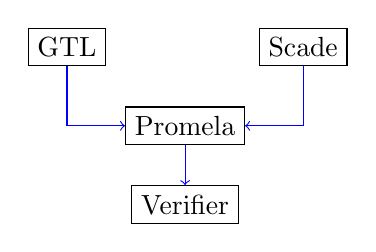
\begin{tikzpicture}
  \node[draw] (promela) at (1.5,1) {Promela};
  \node[draw] (gtl) at (0,2) {GTL};
  \node[draw] (scade) at (3,2) {Scade};
  \node[draw] (verifier) at (1.5,0) {Verifier};
  \draw[->,blue] (scade) |- (promela);
  \draw[->,blue] (gtl) |- (promela);
  \draw[->,blue] (promela) -- (verifier);
\end{tikzpicture}

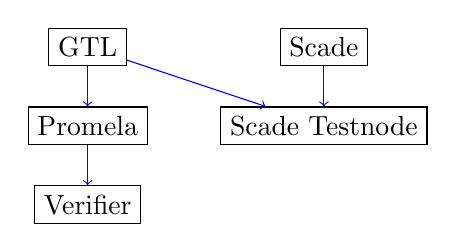
\begin{tikzpicture}
  \node[draw] (gtl) at (0,2) {GTL};
  \node[draw] (scade) at (3,2) {Scade};
  \node[draw] (promela) at (0,1) {Promela};
  \node[draw] (testnode) at (3,1) {Scade Testnode};
  \node[draw] (verifier) at (0,0) {Verifier};
  \draw[->,blue] (gtl) -- (promela);
  \draw[->,blue] (scade) -- (testnode);
  \draw[->,blue] (gtl) -- (testnode);
  \draw[->,blue] (promela) -- (verifier);
\end{tikzpicture}

